\documentclass[11pt, a4paper]{article}
\usepackage[total={7in, 10in}]{geometry}
\usepackage{fullwidth}
\usepackage{hyperref}
\usepackage{tabularx}
\usepackage{graphicx}
\usepackage[normalem]{ulem}


\hypersetup{
    colorlinks=true,
    linkcolor=blue,
    urlcolor=cyan,
}

\graphicspath{ {./asserts/logo/} }

\begin{document}

\begin{center}
    \textbf{{\huge Shrikant Singh}}
\end{center}
\begin{center}
    \begin{tabular}{ c | c | c | c}
        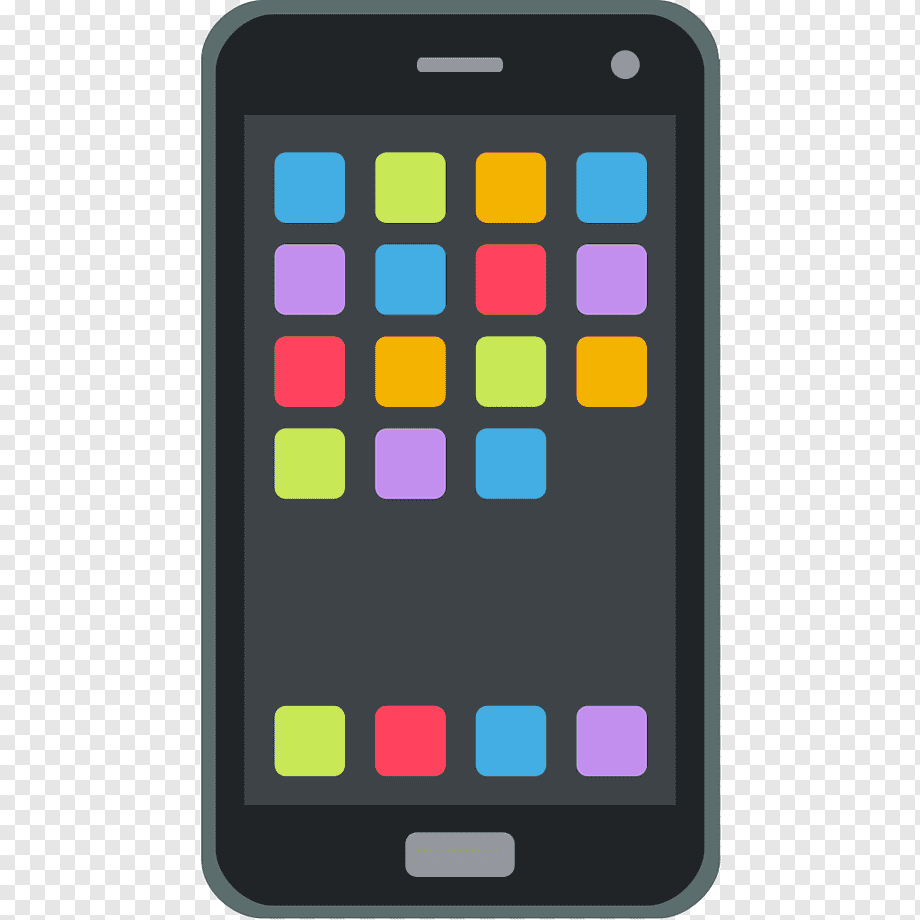
\includegraphics[height=.018\textwidth]{phone} \href{tel:+918010879792}{+91-8010879792} &
        
\includegraphics[height=.018\textwidth]{gmail} \href{mailto:thisshri@gmail.com} {thisshri@gmail.com} &
        
\includegraphics[height=.018\textwidth]{web} \href{https://shrikantsingh.com} {shrikantsingh.com}&
        
\includegraphics[height=.018\textwidth]{github} \href{https://github.com/thisshri} {thisshri} \\
    \end{tabular}
\end{center}

\begin{flushleft}
    \uline{\textsc{\large{\textbf{Summary}}}\hfill}
    \newline
    \newline
    Software developer with 3+ years of experience building various types of products using popular technologies like ReactJs, NodeJs, and Django. Strong creative and analytical skills.
\end{flushleft}

\setlength\tabcolsep{0pt}
\begin{flushleft}
    \uline{\textsc{\large{\textbf{Experience}}}\hfill}
    \newline
    \newline
\setlength\tabcolsep{0pt}
\begin{tabularx}{\textwidth}{X r}
    \large{\textbf{2.) Str8bat}} & Bangalore, India\\
    \textit{Software Developer} & \textit {Sept, 2020 - Present}\\
\end{tabularx}
\begin{itemize}
    \textbf{Str8bat uses IoT based technology that gives real-time actionable insights to budding and professional cricket batters.
    }

    \textbf{Responsible}
    for the whole backend development, related integration with other platforms like SendGrid, MSG91, google, and apple for subscription-related things, mentoring juniors, interns, and everything else that comes with working in a small team startup.

    \item {\bf{Str8bat - Backend}}
    \newline
    Heavily involved in the SDLC process to develop and maintain the core backend for the str8bat app, including everything from user login to user subscription for android and iPhone users.
    Working closely with the CEO to discuss design and develop str8bat backend to increase user engagement.
    \newline
    \textbf{Tech}: Node, Express, React, AntDesign, Less, Redux Loop, Postgres, Knex. 
    \item {\bf{GetBetter}}
    \newline
    Designed and developed \href{https://getbetter.str8bat.com}{getbetter.str8bat.com}, an event booking platform to book coaching sessions by professional cricketers.
    \newline
    \textbf{Tech}: Django, Razorpay, and Stripe.
    \item {\bf{Admin Dashboard}}
    \newline
    Built and maintaining a platform used by str8bat internal team to CRUD data related to our str8bat platform.
    \newline
    \textbf{Tech}: React, AntDesign, Sess, and Redux Loop. 

\end{itemize}

    \begin{tabularx}{\textwidth}{X r}
        \large{\textbf{1.) Delinno}} & Gurgaon, India\\
        \textit{Software Developer}  & \textit {Feb, 2019 - May, 2020}\\
    \end{tabularx}
\end{flushleft}

\begin{flushleft}
\begin{itemize}
    \item {\bf{Digital CSR Platform}}
    \newline
    \textbf{Responsibilites:} Add new features, fix bugs, refactor existing code to improve code quality, and refactor mobile app UI by removing antd mobile and using antd so that it looks good on the desktop as well as on mobile platform.
    \newline
    \textbf{Tech}: Node, Express, React, AntDesign, Less, Redux Loop, Postgres, Knex. 

    \item \textbf{Online Fitness Course Platform}
    \newline
    \textbf{Responsibilites:} Started the project from scratch, Lead a team of 3, flesh out tasks/ features for the team members, review code to maintain consistency, and quality code.
    \newline
    \textbf{Tech}: Python, Django, React, MaterialUI, Redux Loop.

    \item \textbf{Online Survey Platform}
    \newline
    \textbf{Responsibilites:} I was a part of a small team and worked on to bump up the React version of the existing custom component library which was used for admin and user app, Porting survey dashboard app from Backbone to React.
    \newline
    \textbf{Tech}: Python, Django, React, Backbone, Redux Loop.

    \item \textbf{Gym CRM}
    \newline
    \textbf{Responsibilites:} Enforce Eslint in the project, GitLabs CI Setup, fix bugs, write API tests, and add new features requested by the client.
    \newline
    \textbf{Tech}: Python, Django, React, AntDesign, Redux Thunk.
    \newline
\end{itemize}

\end{flushleft}

\begin{flushleft}
    \uline{\textsc{\large{\textbf{Skills}}}\hfill}
    \newline
    \newline
    \begin{tabular}{l l}
        \textbf{Fontend: } & HTML, CSS, Scss, JavaScript, React, Redux.\\
        \textbf{UI Libraries: } & AntDesign, MaterialUI, ReactBootstrap.\\
        \textbf{Backend: } & NodeJs, Django.\\
        \textbf{Database: } & Postgres, Knex.\\
        \textbf{Other: } & Git, VIM, Latex, CI/CD, and AWS-EC2\\
    \end{tabular}
    \newline
\end{flushleft}

\begin{flushleft}
    \uline{\textsc{\large{\textbf{Education}}}\hfill}
    \newline
    \newline
    \setlength\tabcolsep{0pt}
    \begin{tabularx}{\textwidth}{X r}
        \large{\textbf{SGTB Khalsa College, University of Delhi}} & Delhi, India \\
        \textit{B.Tech in Computer Science} & \textit{Aug, 2013 - Aug, 2017} \\
    \end{tabularx}
    \newline
\end{flushleft}

\end{document}
